To evaluate the accuracy of the \osprey \ks algorithm~\cite{K*}, we performed a series of designs for a variety of protein-protein interfaces (PPIs) as retrospective validation. We used \ks to computationally predict experimentally measured changes in binding for each PPI. Each protein structure is listed by name and PDB ID in Table \ref{table:spearman} \cite{pdb1x1u,pdb2pcb,pdb3s9d,pdb2b5i}.  These systems include barnase with its peptide inhibitor barstar \cite{binding2barnase,bindingbarnase}, the cytochrome {\it c}:cytochrome {\it c} peroxidase complex \cite{bindingcytc}, interferon (IFN)$\alpha$2 with its receptor, ifnar2  \cite{bindingifna2}, and the interleukin 2 (IL-2):IL-2 receptor $\alpha$ (IL-2R$\alpha$) complex \cite{bindingil2}.

Our retrospective validation experiments focused on mutations at residues in or proximal to the protein-protein interface that were not limited to alanine scanning. Including some of these tested and reported mutations \cite{binding2barnase,bindingbarnase,bindingcytc,bindingifna2,bindingil2}, for each structure we tested anywhere from 5 to 19 designs. In total, we tested 58 mutations using default, out-of-the-box \osprey settings and parameters. Each design included one or two mutable residues along with a set of surrounding flexible residues (See Table \ref{table:spearman}). Flexible residues were chosen by selecting all residues within 4{\AA} of the mutable residues and removing those which only have backbone interactions. Two example designs are shown in Figure \ref{fig:designs}. For each system, the \ks scores were ranked in increasing order of reported experimental binding. Spearman's $\rho$ values were subsequently calculated for each system by calculating the statistical dependence between the \ks score rankings and the experimentally measured rankings (Table \ref{table:spearman}). 

\begin{figure}
 \center
 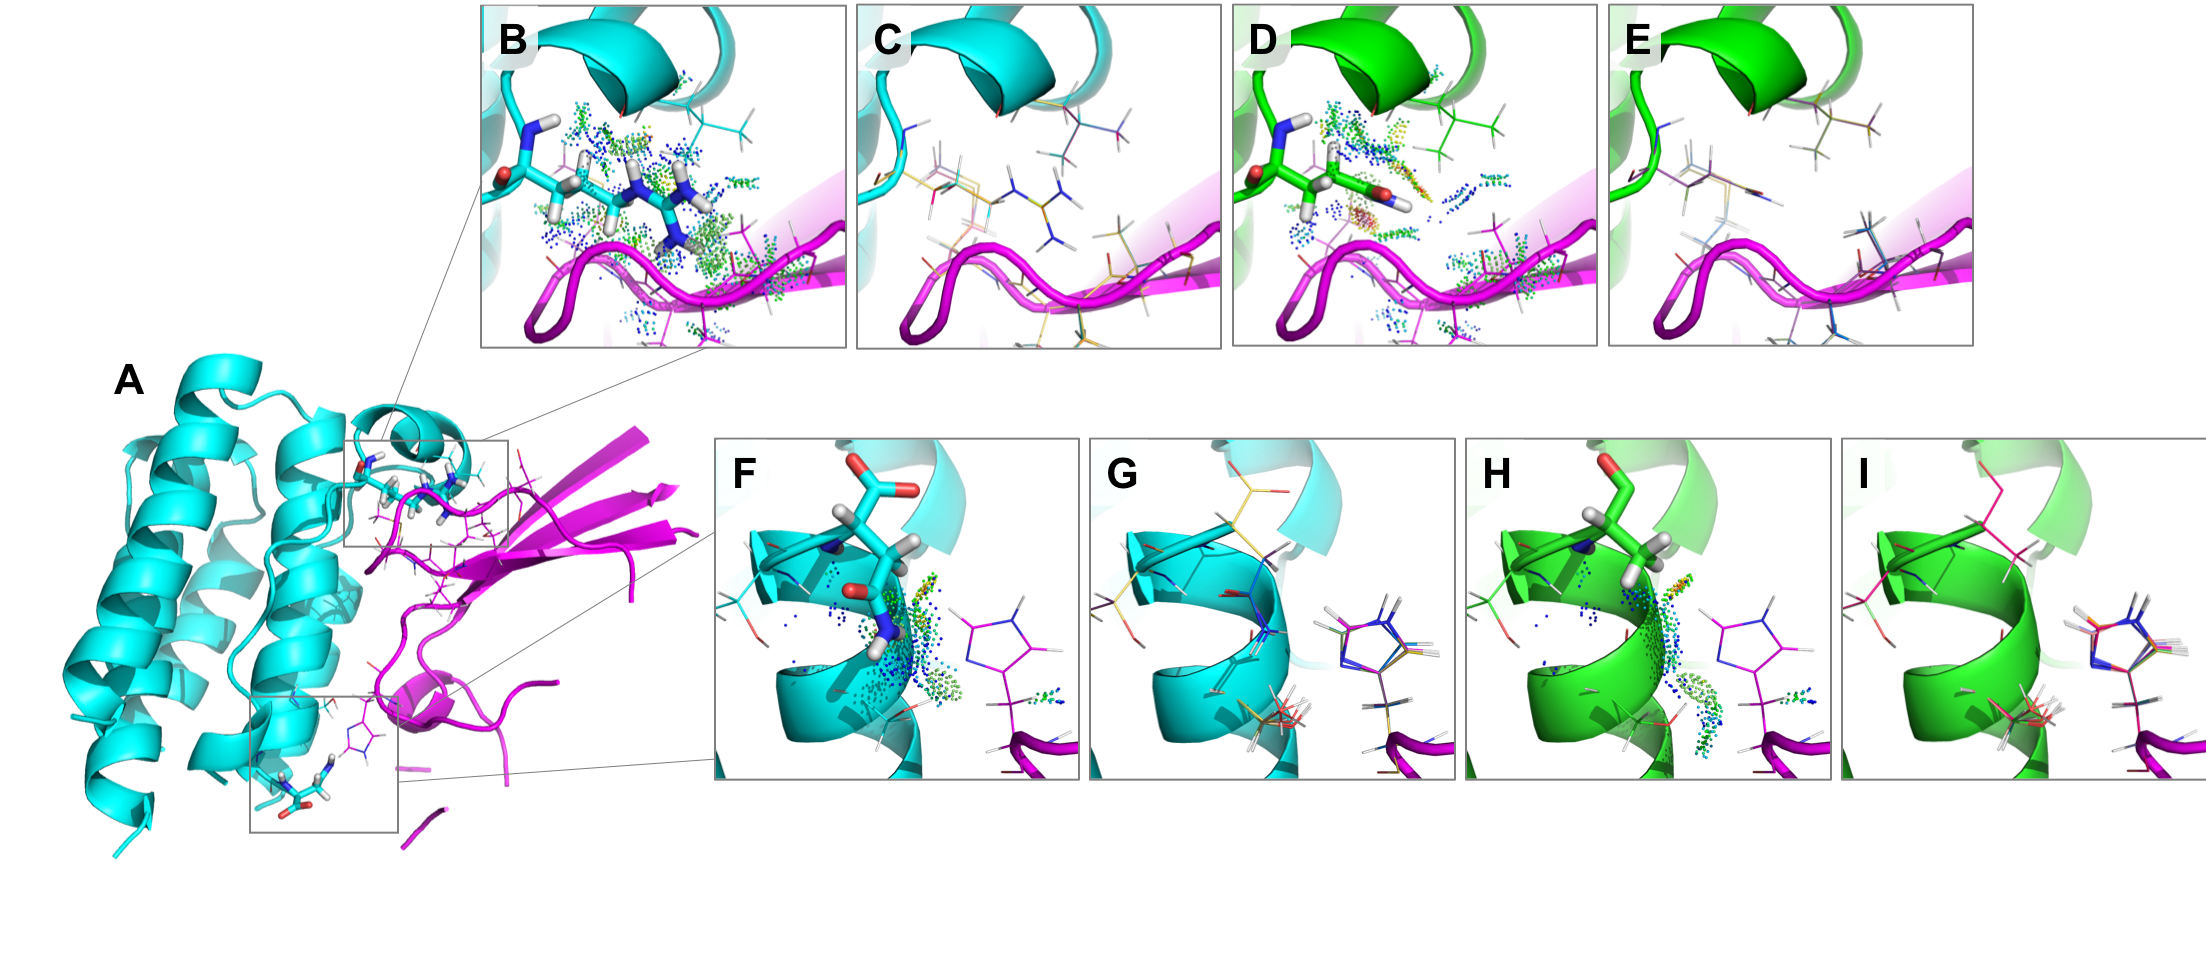
\includegraphics[width=\textwidth]{figures/designExamples.png}
 \caption{(A) The structure of the IFN$\alpha$2:IFNAR2 complex (PDB ID: 3S9D \cite{pdb3s9d}) with separate chains shown in cyan and magenta and with two example interface design regions shown in boxes. Each box contains a mutable residue shown as sticks and its surrounding flexible residues shown as lines. (B) and (F) zoom in on each design. (B-D) Design at position R33 for a mutation that decreases binding: R33Q. (B) The wildtype sequence with probe dots \cite{Probe} displaying favorable interactions with surrounding flexible residues (shown as lines). (D) The mutant sequence (R33Q) with probe dots displaying some favorable as well as unfavorable interactions. Comparing (B) and (D), it is clear there is a loss in favorable interactions and a gain in unfavorable interactions upon mutation from R to Q; this behavior is captured accurately by the \ks algorithm (See Table \ref{table:spearman}). (C) \& (E) The top 10 conformations found in the conformational ensemble used in the \ks calculation for each sequence. (F-I) Design at position N156 for a mutation that increases binding: N156A. (F) The wildtype sequence with probe dots displaying some favorable interactions with surrounding flexible residues (shown as lines). (H) The mutant sequence (N156A) with probe dots displaying some favorable interactions with surrounding flexible residues (shown as lines). There are some gained interactions in (H) compared to (F), but these are not easily detected, thus emphasizing the importance of \ks, which successfully picks up these nuanced changes and correctly predicts improved binding (See Table \ref{table:spearman}). (G) and (I) show the top 10 conformations found in the conformational ensemble used in the \ks calculation for each sequence. Not shown are the ensembles for the unbound states that are also used to calculate the \ks scores.}
\label{fig:designs}
\end{figure}

\begin{table}[h]
\centering
\scriptsize
\resizebox{.49\linewidth}{!}{
\begin{tabular}{|K{1.3cm}|K{1.7cm}|K{2cm}|K{2cm}|}
\hline
 & Mutation(s) & Experimental Ranking & Computational Ranking\\
\hline
\parbox[t]{2mm}{\multirow{13}{*}{\rotatebox[origin=c]{90}{Barnase:Barstar, PDB ID: 1X1U}}} & D39A & 1 & 1\\
 & H102A & 2 & 3\\
 & R87A & 3 & 5\\
 & K27A & 4 & 8\\
 & R59A & 5 & 2\\
 & D35A & 6 & 4\\
 & Y29A & 7 & 7\\
 & E73A & 8 & 12\\
 & E76A & 9 & 6\\
 & W35F & 10 & 11\\
 & E60A & 11 & 10\\
 & Y29F & 12 & 9\\ \cline{3-4}
 && \multicolumn{2}{c|}{$\rho = 0.755$} \\
\hline
\parbox[t]{2mm}{\multirow{17}{*}{\rotatebox[origin=c]{90}{IL-2:IL-2R$\alpha$, PDB ID: 2B5I}}} & K38E, S39D & 1.5 & 1\\
 & R35T, R36S & 1.5 & 2\\
 & R35K, R36K & 3 & 4\\
 & E1K, D4K & 4 & 7\\
 & E29R & 5 & 5\\
 & L2A & 6 & 16\\
 & D4K & 7.5 & 9\\
 & S39A, S41A & 7.5 & 12\\
 & E1K & 9 & 11\\
 & H120A & 10 & 10\\
 & E29A & 11 & 6\\
 & L42S, Y43L & 12 & 3\\
 & E1Q & 13 & 14\\
 & N27A & 14 & 15\\
 & K38T & 15 & 8\\
 & D4N & 16 & 13\\ \cline{3-4} 
 && \multicolumn{2}{c|}{$\rho = 0.554$}  \\
\hline
\end{tabular}
}
\resizebox{.49\linewidth}{!}{
\begin{tabular}{|K{1.3cm}|K{1.7cm}|K{2cm}|K{2cm}|}
\hline
\multirow{6}{*}{\rotatebox[origin=c]{90}{\parbox[t]{2.5cm}{\centering Cyt{\it{c}}:Cyt{\it{c}} peroxidase, PDB ID: 2PCB}}} & E290N & 1 & 2\\
 & D34N & 2 & 4\\
 & A193F & 3 & 1\\
 & E35Q & 4 & 3\\ 
 & E32Q & 5 & 5\\ \cline{3-4}
 && \multicolumn{2}{c|}{$\rho = 0.500$} \\ 
\hline
\parbox[t]{2mm}{\multirow{20}{*}{\rotatebox[origin=c]{90}{IFN$\alpha$2:ifnar2, PDB ID: 3S9D}}} & \colorbox{LightCyan}{R33Q} & 1 & 1\\
 & R33A & 2 & 2\\
 & R33K & 3 & 5\\
 & L30A & 4 & 6\\
 & R149A & 5 & 4\\
 & L30V & 6 & 9\\
 & A148A & 7 & 10\\
 & A145G & 8 & 14\\
 & A145M & 9 & 3\\
 & L15A & 10 & 13\\
 & L153A & 11 & 12\\
 & L26A & 12 & 7\\
 & S152A & 13 & 16\\
 & F27A & 14 & 8\\
 & S25A & 15 & 18\\
 & D35A & 16 & 17\\
 & R22A & 17 & 11\\
 & M16A & 18 & 15\\
 & \colorbox{LightCyan}{N156A} & 19 & 19\\ \cline{3-4}
 && \multicolumn{2}{c|}{$\rho = 0.795$} \\
 \hline
 \multicolumn{2}{|c|}{} & {\textbf{Across All}} & $\rho = 0.762$ \\
\hline
\end{tabular}
}
\caption{Allowed mutations for each system are listed along with their corresponding rankings from experimental \cite{binding2barnase,bindingbarnase,bindingcytc,bindingifna2,bindingil2} and computational results. The mutations highlighted in blue are shown in detail in Figure \ref{fig:designs}. A Spearman's $\rho$ value is calculated for each system and shown here. The ``Across All" value is calculated by ranking each system individually and then calculating the Spearman's $\rho$ across all of the designs---in other words, it is the Pearson correlation of the intra-system ranks of all the mutants.  We consider this meaningful because the output of a design calculation that is used to decide on mutants to make experimentally is simply the intra-system ranks of the mutants.}
\label{table:spearman}
\end{table}

\begin{figure}
\center
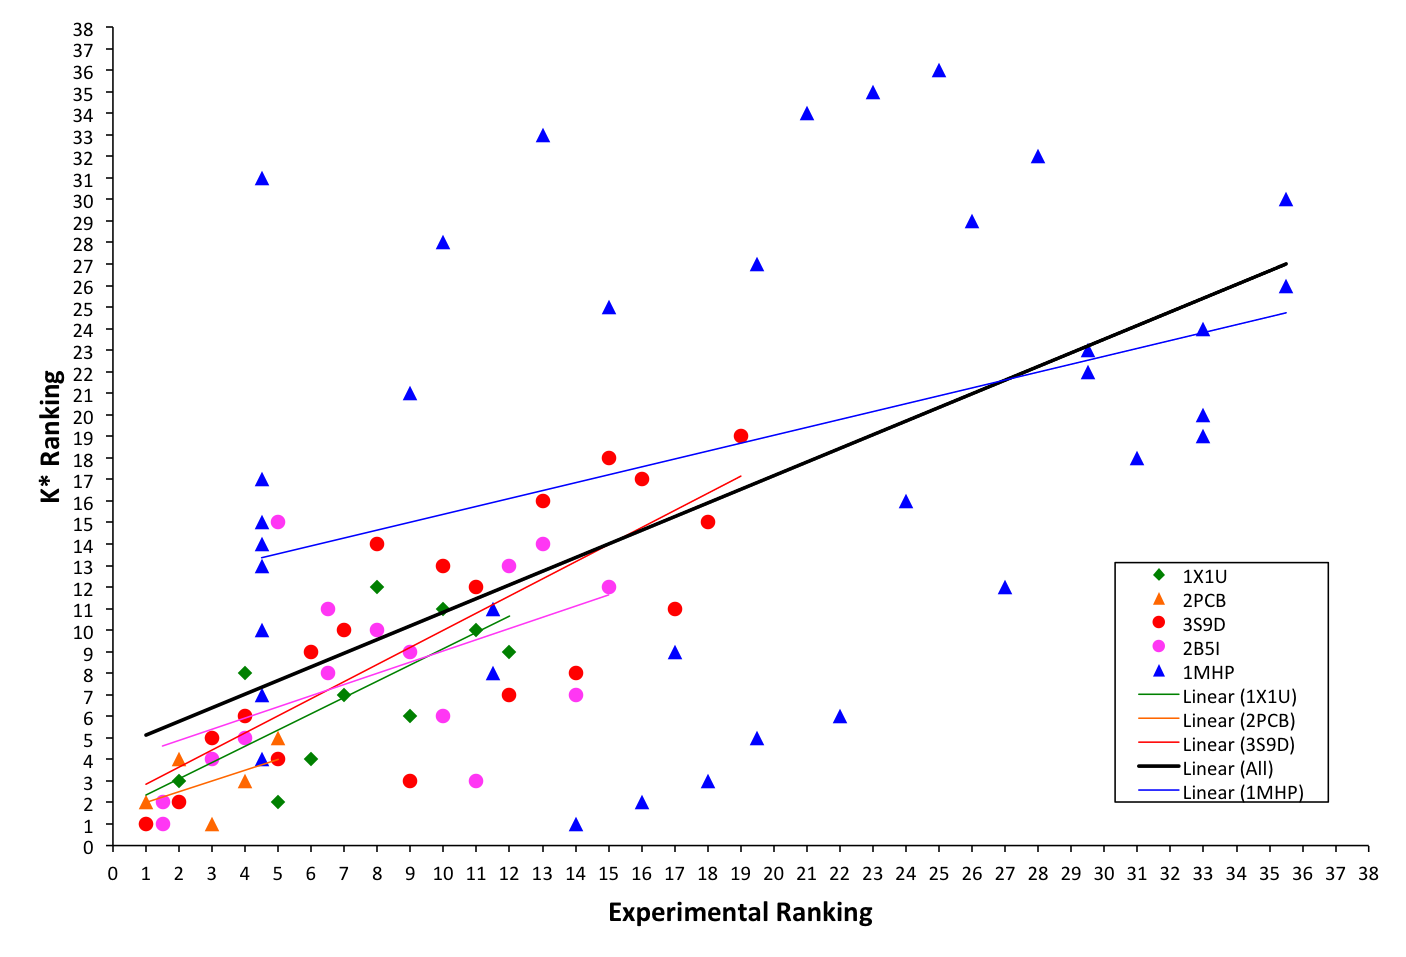
\includegraphics[width=0.9\textwidth]{figures/Rankings.png}
\caption{Testing the accuracy of the \ks algorithm in \osprey3 by comparing \ks rankings to experimentally reported rankings (See Table \ref{table:spearman}). Each system is represented by its corresponding PDB ID and a linear trendline is shown for each in its corresponding color according to the legend.}
\label{fig:rankings}
\end{figure}

% \begin{table}[h!]\label{table:spearman}
% \centering
% \begin{tabular}{ |c||c|  }
%  \hline
%  \textbf{Structures (PDB ID)}& \textbf{Spearman's $\rho$} \\
%  \hline 
%  3S9D   & 0.795 \\
%  \hline
%  1X1U   & 0.755 \\
%  \hline
%  2B5I   & 0.554 \\
%  \hline
%  2PCB   & 0.500 \\
%  \hline
%  \textbf{Across Structures} &   \textbf{0.762}  \\
%  \hline
% \end{tabular}
% \caption{Spearman's $\rho$ table. A Spearman's $\rho$ value is calculated for each system and shown here. The ``Across Structures" value is calculated by ranking each system individually and then calculating the Spearman's $\rho$ across all of the designs---in other words, it is the Pearson correlation of the intra-system ranks of all the mutants.  We consider this meaningful because the output of a design calculation that is used to decide on mutants to make experimentally is simply the intra-system ranks of the mutants.  }
% \end{table}
